%----------------------------------------------------------------------------------------
%	PACKAGES AND OTHER DOCUMENT CONFIGURATIONS
%----------------------------------------------------------------------------------------

\documentclass[11pt,a4paper]{book} % Default font size and left-justified equations
\usepackage[x11names,svgnames,dvipsnames]{xcolor}
\everymath{\displaystyle}
\usepackage[cal=boondoxo]{mathalfa} % mathcal
\usepackage{amssymb,amsmath}
\usepackage{mathtools}
\usepackage{amsfonts}
\usepackage{amsthm}
\usepackage{palatino}
\usepackage{mathpazo}
\usepackage{tikz}%for draw
\usepackage{wrapfig}
\usetikzlibrary{mindmap} % LATEX and plain TEX
\usepgflibrary{decorations.text} % LATEX and plain TEX and pure pgf 
\usepgflibrary[decorations.text] % ConTEXt and pure pgf 
\usetikzlibrary{decorations.text} % LATEX and plain TEX when using TikZ 
\usetikzlibrary[decorations.text] % ConTEXt when using TikZ
\usetikzlibrary{automata} % LATEX and plain TEX
\usetikzlibrary[automata] % ConTEXt
%\setmainfont[Scale = 0.84, Script=Khmer] {Khmer OS System}
%----------------------------------------------------------------------------------------
%	VARIOUS REQUIRED PACKAGES AND CONFIGURATIONS
%----------------------------------------------------------------------------------------

\usepackage[top=3cm,bottom=3cm,left=3cm,right=3cm,headsep=10pt,a4paper]{geometry} % Page margins

\usepackage{graphicx} % Required for including pictures
\graphicspath{{Pictures/}} % Specifies the directory where pictures are stored

\usepackage{lipsum} % Inserts dummy text

\usepackage{tikz} % Required for drawing custom shapes

\usepackage[english]{babel} % English language/hyphenation

\usepackage{enumitem} % Customize lists
\setlist{nolistsep} % Reduce spacing between bullet points and numbered lists

\usepackage{booktabs} % Required for nicer horizontal rules in tables

\usepackage{xcolor} % Required for specifying colors by name
\definecolor{ocre}{RGB}{243,102,25} % Define the orange color used for highlighting throughout the book

%----------------------------------------------------------------------------------------
%	FONTS
%----------------------------------------------------------------------------------------

\usepackage{avant} % Use the Avantgarde font for headings
%\usepackage{times} % Use the Times font for headings
\usepackage{mathptmx} % Use the Adobe Times Roman as the default text font together with math symbols from the Sym­bol, Chancery and Com­puter Modern fonts

\usepackage{microtype} % Slightly tweak font spacing for aesthetics
\usepackage[utf8]{inputenc} % Required for including letters with accents
\usepackage[T1]{fontenc} % Use 8-bit encoding that has 256 glyphs

%----------------------------------------------------------------------------------------
%	BIBLIOGRAPHY AND INDEX
%----------------------------------------------------------------------------------------

\usepackage{csquotes}
\usepackage[style=alphabetic,citestyle=numeric,sorting=nyt,sortcites=true,autopunct=true,autolang=hyphen,hyperref=true,abbreviate=false,backref=true,backend=biber,defernumbers=true]{biblatex}
\addbibresource{bibliography.bib} % BibTeX bibliography file
\defbibheading{bibempty}{}

\usepackage{calc} % For simpler calculation - used for spacing the index letter headings correctly
\usepackage{makeidx} % Required to make an index
\makeindex % Tells LaTeX to create the files required for indexing

%----------------------------------------------------------------------------------------
%	MAIN TABLE OF CONTENTS
%----------------------------------------------------------------------------------------

\usepackage{titletoc} % Required for manipulating the table of contents

\contentsmargin{0cm} % Removes the default margin

% Part text styling
\titlecontents{part}[0cm]
{\addvspace{20pt}\centering\large\bfseries}
{}
{}
{}

% Chapter text styling
\titlecontents{chapter}[1.25cm] % Indentation
{\addvspace{12pt}\large\sffamily\bfseries} % Spacing and font options for chapters
{\color{ocre!60}\contentslabel[\Large\thecontentslabel]{1.25cm}\color{ocre}} % Chapter number
{\color{ocre}}  
{\color{ocre!60}\normalsize\;\titlerule*[.5pc]{.}\;\thecontentspage} % Page number

% Section text styling
\titlecontents{section}[1.25cm] % Indentation
{\addvspace{3pt}\sffamily\bfseries} % Spacing and font options for sections
{\contentslabel[\thecontentslabel]{1.25cm}} % Section number
{}
{\hfill\color{black}\thecontentspage} % Page number
[]

% Subsection text styling
\titlecontents{subsection}[1.25cm] % Indentation
{\addvspace{1pt}\sffamily\small} % Spacing and font options for subsections
{\contentslabel[\thecontentslabel]{1.25cm}} % Subsection number
{}
{\ \titlerule*[.5pc]{.}\;\thecontentspage} % Page number
[]

% List of figures
\titlecontents{figure}[0em]
{\addvspace{-5pt}\sffamily}
{\thecontentslabel\hspace*{1em}}
{}
{\ \titlerule*[.5pc]{.}\;\thecontentspage}
[]

% List of tables
\titlecontents{table}[0em]
{\addvspace{-5pt}\sffamily}
{\thecontentslabel\hspace*{1em}}
{}
{\ \titlerule*[.5pc]{.}\;\thecontentspage}
[]

%----------------------------------------------------------------------------------------
%	MINI TABLE OF CONTENTS IN PART HEADS
%----------------------------------------------------------------------------------------

% Chapter text styling
\titlecontents{lchapter}[0em] % Indenting
{\addvspace{15pt}\large\sffamily\bfseries} % Spacing and font options for chapters
{\color{ocre}\contentslabel[\Large\thecontentslabel]{1.25cm}\color{ocre}} % Chapter number
{}  
{\color{ocre}\normalsize\sffamily\bfseries\;\titlerule*[.5pc]{.}\;\thecontentspage} % Page number

% Section text styling
\titlecontents{lsection}[0em] % Indenting
{\sffamily\small} % Spacing and font options for sections
{\contentslabel[\thecontentslabel]{1.25cm}} % Section number
{}
{}

% Subsection text styling
\titlecontents{lsubsection}[.5em] % Indentation
{\normalfont\footnotesize\sffamily} % Font settings
{}
{}
{}

%----------------------------------------------------------------------------------------
%	PAGE HEADERS
%----------------------------------------------------------------------------------------

\usepackage{fancyhdr} % Required for header and footer configuration

\pagestyle{fancy}
\renewcommand{\chaptermark}[1]{\markboth{\sffamily\normalsize\bfseries\chaptername\ \thechapter.\ #1}{}} % Chapter text font settings
\renewcommand{\sectionmark}[1]{\markright{\sffamily\normalsize\thesection\hspace{5pt}#1}{}} % Section text font settings
\fancyhf{} \fancyhead[LE,RO]{\sffamily\normalsize\thepage} % Font setting for the page number in the header
\fancyhead[LO]{\rightmark} % Print the nearest section name on the left side of odd pages
\fancyhead[RE]{\leftmark} % Print the current chapter name on the right side of even pages
\renewcommand{\headrulewidth}{0.5pt} % Width of the rule under the header
\addtolength{\headheight}{2.5pt} % Increase the spacing around the header slightly
\renewcommand{\footrulewidth}{0pt} % Removes the rule in the footer
\fancypagestyle{plain}{\fancyhead{}\renewcommand{\headrulewidth}{0pt}} % Style for when a plain pagestyle is specified

% Removes the header from odd empty pages at the end of chapters
\makeatletter
\renewcommand{\cleardoublepage}{
\clearpage\ifodd\c@page\else
\hbox{}
\vspace*{\fill}
\thispagestyle{empty}
\newpage
\fi}

%----------------------------------------------------------------------------------------
%	THEOREM STYLES
%----------------------------------------------------------------------------------------

\usepackage{amsmath,amsfonts,amssymb,amsthm} % For math equations, theorems, symbols, etc

\newcommand{\intoo}[2]{\mathopen{]}#1\,;#2\mathclose{[}}
\newcommand{\ud}{\mathop{\mathrm{{}d}}\mathopen{}}
\newcommand{\intff}[2]{\mathopen{[}#1\,;#2\mathclose{]}}
\newtheorem{notation}{Notation}[chapter]

% Boxed/framed environments
\newtheoremstyle{ocrenumbox}% % Theorem style name
{0pt}% Space above
{0pt}% Space below
{\normalfont}% % Body font
{}% Indent amount
{\small\bf\sffamily\color{ocre}}% % Theorem head font
{\;}% Punctuation after theorem head
{0.25em}% Space after theorem head
{\small\sffamily\color{ocre}\thmname{#1}\nobreakspace\thmnumber{\@ifnotempty{#1}{}\@upn{#2}}% Theorem text (e.g. Theorem 2.1)
\thmnote{\nobreakspace\the\thm@notefont\sffamily\bfseries\color{black}---\nobreakspace#3.}} % Optional theorem note
\renewcommand{\qedsymbol}{$\blacksquare$}% Optional qed square

\newtheoremstyle{blacknumex}% Theorem style name
{5pt}% Space above
{5pt}% Space below
{\normalfont}% Body font
{} % Indent amount
{\small\bf\sffamily}% Theorem head font
{\;}% Punctuation after theorem head
{0.25em}% Space after theorem head
{\small\sffamily{\tiny\ensuremath{\blacksquare}}\nobreakspace\thmname{#1}\nobreakspace\thmnumber{\@ifnotempty{#1}{}\@upn{#2}}% Theorem text (e.g. Theorem 2.1)
\thmnote{\nobreakspace\the\thm@notefont\sffamily\bfseries---\nobreakspace#3.}}% Optional theorem note

\newtheoremstyle{blacknumbox} % Theorem style name
{0pt}% Space above
{0pt}% Space below
{\normalfont}% Body font
{}% Indent amount
{\small\bf\sffamily}% Theorem head font
{\;}% Punctuation after theorem head
{0.25em}% Space after theorem head
{\small\sffamily\thmname{#1}\nobreakspace\thmnumber{\@ifnotempty{#1}{}\@upn{#2}}% Theorem text (e.g. Theorem 2.1)
\thmnote{\nobreakspace\the\thm@notefont\sffamily\bfseries---\nobreakspace#3.}}% Optional theorem note

% Non-boxed/non-framed environments
\newtheoremstyle{ocrenum}% % Theorem style name
{5pt}% Space above
{5pt}% Space below
{\normalfont}% % Body font
{}% Indent amount
{\small\bf\sffamily\color{ocre}}% % Theorem head font
{\;}% Punctuation after theorem head
{0.25em}% Space after theorem head
{\small\sffamily\color{ocre}\thmname{#1}\nobreakspace\thmnumber{\@ifnotempty{#1}{}\@upn{#2}}% Theorem text (e.g. Theorem 2.1)
\thmnote{\nobreakspace\the\thm@notefont\sffamily\bfseries\color{black}---\nobreakspace#3.}} % Optional theorem note
\renewcommand{\qedsymbol}{$\blacksquare$}% Optional qed square
\makeatother

% Defines the theorem text style for each type of theorem to one of the three styles above
\newcounter{dummy} 
\numberwithin{dummy}{section}
\theoremstyle{ocrenumbox}
\newtheorem{theoremeT}[dummy]{Theorem}
\newtheorem{problem}{Problem}[chapter]
\newtheorem{exerciseT}{Exercise}[chapter]
\theoremstyle{blacknumex}
\newtheorem{exampleT}{Example}[chapter]
\theoremstyle{blacknumbox}
\newtheorem{vocabulary}{Vocabulary}[chapter]
\newtheorem{definitionT}{Definition}[section]
\newtheorem{corollaryT}[dummy]{Corollary}
\theoremstyle{ocrenum}
\newtheorem{proposition}[dummy]{Proposition}

%----------------------------------------------------------------------------------------
%	DEFINITION OF COLORED BOXES
%----------------------------------------------------------------------------------------

\RequirePackage[framemethod=default]{mdframed} % Required for creating the theorem, definition, exercise and corollary boxes

% Theorem box
\newmdenv[skipabove=7pt,
skipbelow=7pt,
backgroundcolor=black!5,
linecolor=ocre,
innerleftmargin=5pt,
innerrightmargin=5pt,
innertopmargin=5pt,
leftmargin=0cm,
rightmargin=0cm,
innerbottommargin=5pt]{tBox}

% Exercise box	  
\newmdenv[skipabove=7pt,
skipbelow=7pt,
rightline=false,
leftline=true,
topline=false,
bottomline=false,
backgroundcolor=ocre!10,
linecolor=ocre,
innerleftmargin=5pt,
innerrightmargin=5pt,
innertopmargin=5pt,
innerbottommargin=5pt,
leftmargin=0cm,
rightmargin=0cm,
linewidth=4pt]{eBox}	

% Definition box
\newmdenv[skipabove=7pt,
skipbelow=7pt,
rightline=false,
leftline=true,
topline=false,
bottomline=false,
linecolor=ocre,
innerleftmargin=5pt,
innerrightmargin=5pt,
innertopmargin=0pt,
leftmargin=0cm,
rightmargin=0cm,
linewidth=4pt,
innerbottommargin=0pt]{dBox}	

% Corollary box
\newmdenv[skipabove=7pt,
skipbelow=7pt,
rightline=false,
leftline=true,
topline=false,
bottomline=false,
linecolor=gray,
backgroundcolor=black!5,
innerleftmargin=5pt,
innerrightmargin=5pt,
innertopmargin=5pt,
leftmargin=0cm,
rightmargin=0cm,
linewidth=4pt,
innerbottommargin=5pt]{cBox}

% Creates an environment for each type of theorem and assigns it a theorem text style from the "Theorem Styles" section above and a colored box from above
\newenvironment{theorem}{\begin{tBox}\begin{theoremeT}}{\end{theoremeT}\end{tBox}}
\newenvironment{exercise}{\begin{eBox}\begin{exerciseT}}{\hfill{\color{ocre}\tiny\ensuremath{\blacksquare}}\end{exerciseT}\end{eBox}}				  
\newenvironment{definition}{\begin{dBox}\begin{definitionT}}{\end{definitionT}\end{dBox}}	
\newenvironment{example}{\begin{exampleT}}{\hfill{\tiny\ensuremath{\blacksquare}}\end{exampleT}}		
\newenvironment{corollary}{\begin{cBox}\begin{corollaryT}}{\end{corollaryT}\end{cBox}}	

%----------------------------------------------------------------------------------------
%	REMARK ENVIRONMENT
%----------------------------------------------------------------------------------------

\newenvironment{remark}{\par\vspace{10pt}\small % Vertical white space above the remark and smaller font size
\begin{list}{}{
\leftmargin=35pt % Indentation on the left
\rightmargin=25pt}\item\ignorespaces % Indentation on the right
\makebox[-2.5pt]{\begin{tikzpicture}[overlay]
\node[draw=ocre!60,line width=1pt,circle,fill=ocre!25,font=\sffamily\bfseries,inner sep=2pt,outer sep=0pt] at (-15pt,0pt){\textcolor{ocre}{R}};\end{tikzpicture}} % Orange R in a circle
\advance\baselineskip -1pt}{\end{list}\vskip5pt} % Tighter line spacing and white space after remark

%----------------------------------------------------------------------------------------
%	SECTION NUMBERING IN THE MARGIN
%----------------------------------------------------------------------------------------

\makeatletter
\renewcommand{\@seccntformat}[1]{\llap{\textcolor{ocre}{\csname the#1\endcsname}\hspace{1em}}}                    
\renewcommand{\section}{\@startsection{section}{1}{\z@}
{-4ex \@plus -1ex \@minus -.4ex}
{1ex \@plus.2ex }
{\normalfont\large\sffamily\bfseries}}
\renewcommand{\subsection}{\@startsection {subsection}{2}{\z@}
{-3ex \@plus -0.1ex \@minus -.4ex}
{0.5ex \@plus.2ex }
{\normalfont\sffamily\bfseries}}
\renewcommand{\subsubsection}{\@startsection {subsubsection}{3}{\z@}
{-2ex \@plus -0.1ex \@minus -.2ex}
{.2ex \@plus.2ex }
{\normalfont\small\sffamily\bfseries}}                        
\renewcommand\paragraph{\@startsection{paragraph}{4}{\z@}
{-2ex \@plus-.2ex \@minus .2ex}
{.1ex}
{\normalfont\small\sffamily\bfseries}}

%----------------------------------------------------------------------------------------
%	PART HEADINGS
%----------------------------------------------------------------------------------------

% numbered part in the table of contents
\newcommand{\@mypartnumtocformat}[2]{%
\setlength\fboxsep{0pt}%
\noindent\colorbox{ocre!20}{\strut\parbox[c][.7cm]{\ecart}{\color{ocre!70}\Large\sffamily\bfseries\centering#1}}\hskip\esp\colorbox{ocre!40}{\strut\parbox[c][.7cm]{\linewidth-\ecart-\esp}{\Large\sffamily\centering#2}}}%
%%%%%%%%%%%%%%%%%%%%%%%%%%%%%%%%%%
% unnumbered part in the table of contents
\newcommand{\@myparttocformat}[1]{%
\setlength\fboxsep{0pt}%
\noindent\colorbox{ocre!40}{\strut\parbox[c][.7cm]{\linewidth}{\Large\sffamily\centering#1}}}%
%%%%%%%%%%%%%%%%%%%%%%%%%%%%%%%%%%
\newlength\esp
\setlength\esp{4pt}
\newlength\ecart
\setlength\ecart{1.2cm-\esp}
\newcommand{\thepartimage}{}%
\newcommand{\partimage}[1]{\renewcommand{\thepartimage}{#1}}%
\def\@part[#1]#2{%
\ifnum \c@secnumdepth >-2\relax%
\refstepcounter{part}%
\addcontentsline{toc}{part}{\texorpdfstring{\protect\@mypartnumtocformat{\thepart}{#1}}{\partname~\thepart\ ---\ #1}}
\else%
\addcontentsline{toc}{part}{\texorpdfstring{\protect\@myparttocformat{#1}}{#1}}%
\fi%
\startcontents%
\markboth{}{}%
{\thispagestyle{empty}%
\begin{tikzpicture}[remember picture,overlay]%
\node at (current page.north west){\begin{tikzpicture}[remember picture,overlay]%	
\fill[ocre!20](0cm,0cm) rectangle (\paperwidth,-\paperheight);
\node[anchor=north] at (4cm,-3.25cm){\color{ocre!40}\fontsize{220}{100}\sffamily\bfseries\@Roman\c@part}; 
\node[anchor=south east] at (\paperwidth-1cm,-\paperheight+1cm){\parbox[t][][t]{8.5cm}{
\printcontents{l}{0}{\setcounter{tocdepth}{1}}%
}};
\node[anchor=north east] at (\paperwidth-1.5cm,-3.25cm){\parbox[t][][t]{15cm}{\strut\raggedleft\color{white}\fontsize{30}{30}\sffamily\bfseries#2}};
\end{tikzpicture}};
\end{tikzpicture}}%
\@endpart}
\def\@spart#1{%
\startcontents%
\phantomsection
{\thispagestyle{empty}%
\begin{tikzpicture}[remember picture,overlay]%
\node at (current page.north west){\begin{tikzpicture}[remember picture,overlay]%	
\fill[ocre!20](0cm,0cm) rectangle (\paperwidth,-\paperheight);
\node[anchor=north east] at (\paperwidth-1.5cm,-3.25cm){\parbox[t][][t]{15cm}{\strut\raggedleft\color{white}\fontsize{30}{30}\sffamily\bfseries#1}};
\end{tikzpicture}};
\end{tikzpicture}}
\addcontentsline{toc}{part}{\texorpdfstring{%
\setlength\fboxsep{0pt}%
\noindent\protect\colorbox{ocre!40}{\strut\protect\parbox[c][.7cm]{\linewidth}{\Large\sffamily\protect\centering #1\quad\mbox{}}}}{#1}}%
\@endpart}
\def\@endpart{\vfil\newpage
\if@twoside
\if@openright
\null
\thispagestyle{empty}%
\newpage
\fi
\fi
\if@tempswa
\twocolumn
\fi}

%----------------------------------------------------------------------------------------
%	CHAPTER HEADINGS
%----------------------------------------------------------------------------------------

% A switch to conditionally include a picture, implemented by  Christian Hupfer
\newif\ifusechapterimage
\usechapterimagetrue
\newcommand{\thechapterimage}{}%
\newcommand{\chapterimage}[1]{\ifusechapterimage\renewcommand{\thechapterimage}{#1}\fi}%
\def\@makechapterhead#1{%
{\parindent \z@ \raggedright \normalfont
\ifnum \c@secnumdepth >\m@ne
\if@mainmatter
\begin{tikzpicture}[remember picture,overlay]
\node at (current page.north west)
{\begin{tikzpicture}[remember picture,overlay]
\node[anchor=north west,inner sep=0pt] at (0,0) {\ifusechapterimage\includegraphics[width=\paperwidth]{\thechapterimage}\fi};
\draw[anchor=west] (\Gm@lmargin,-9cm) node [line width=2pt,rounded corners=15pt,draw=ocre,fill=white,fill opacity=0.5,inner sep=15pt]{\strut\makebox[22cm]{}};
\draw[anchor=west] (\Gm@lmargin+.3cm,-9cm) node {\huge\sffamily\bfseries\color{black}\thechapter. #1\strut};
\end{tikzpicture}};
\end{tikzpicture}
\else
\begin{tikzpicture}[remember picture,overlay]
\node at (current page.north west)
{\begin{tikzpicture}[remember picture,overlay]
\node[anchor=north west,inner sep=0pt] at (0,0) {\ifusechapterimage\includegraphics[width=\paperwidth]{\thechapterimage}\fi};
\draw[anchor=west] (\Gm@lmargin,-9cm) node [line width=2pt,rounded corners=15pt,draw=ocre,fill=white,fill opacity=0.5,inner sep=15pt]{\strut\makebox[22cm]{}};
\draw[anchor=west] (\Gm@lmargin+.3cm,-9cm) node {\huge\sffamily\bfseries\color{black}#1\strut};
\end{tikzpicture}};
\end{tikzpicture}
\fi\fi\par\vspace*{270\p@}}}

%-------------------------------------------

\def\@makeschapterhead#1{%
\begin{tikzpicture}[remember picture,overlay]
\node at (current page.north west)
{\begin{tikzpicture}[remember picture,overlay]
\node[anchor=north west,inner sep=0pt] at (0,0) {\ifusechapterimage\includegraphics[width=\paperwidth]{\thechapterimage}\fi};
\draw[anchor=west] (\Gm@lmargin,-9cm) node [line width=2pt,rounded corners=15pt,draw=ocre,fill=white,fill opacity=0.5,inner sep=15pt]{\strut\makebox[22cm]{}};
\draw[anchor=west] (\Gm@lmargin+.3cm,-9cm) node {\huge\sffamily\bfseries\color{black}#1\strut};
\end{tikzpicture}};
\end{tikzpicture}
\par\vspace*{270\p@}}
\makeatother

%----------------------------------------------------------------------------------------
%	HYPERLINKS IN THE DOCUMENTS
%----------------------------------------------------------------------------------------

\usepackage{hyperref}
\hypersetup{hidelinks,colorlinks=false,breaklinks=true,urlcolor= ocre,bookmarksopen=false,pdftitle={Title},pdfauthor={Author}}
\usepackage{bookmark}
\bookmarksetup{
open,
numbered,
addtohook={%
\ifnum\bookmarkget{level}=0 % chapter
\bookmarksetup{bold}%
\fi
\ifnum\bookmarkget{level}=-1 % part
\bookmarksetup{color=ocre,bold}%
\fi
}
}
 % Insert the commands.tex file which contains the majority of the structure behind the template
\usepackage{fontspec}
\setmainfont{Times New Roman}
\newcommand{\en}{\fontspec{Times New Roman}\selectfont}
\newcommand{\enb}{\fontspec[Color=Blue]{Times New Roman}\selectfont}
\newcommand{\red}{\fontspec[Color=Red]{Times New Roman}\selectfont}
\newcommand{\m }{\fontspec{Menlo}\selectfont}
\newcommand{\mb}{\fontspec[Color=Blue]{Menlo}\selectfont}
\newcommand{\mg}{\fontspec[Color=PineGreen]{Menlo}\selectfont}
\newcommand{\mo}{\fontspec[Color=Orange]{Menlo}\selectfont}
\newcommand{\cnr}{\fontspec[Color=Red]{Courier New}\selectfont}
\newcommand{\cnp}{\fontspec[Color=Plum]{Courier New}\selectfont}
%===========KHMER FONT=======================
\newfontfamily\khmerfamily[Scale=0.8,Script=Khmer]{Khmer OS Moul}
\newcommand{\khl}{\fontspec[Scale=0.84,Script=Khmer,Color=Blue]{Khmer OS Moul}\selectfont} 
\newcommand{\khlw}{\fontspec[Scale=0.84,Script=Khmer,Color=Yellow]{Khmer OS Moul}\selectfont} 
\newfontfamily\khmerfamily[Scale=0.8,Script=Khmer]{Ang DaunTeav}
\newcommand{\ad}{\fontspec[Scale=0.84,Script=Khmer]{Ang DaunTeav}\selectfont}

%=============END KHMER FONT FOR BOOK===============
%\hypersetup{pdftitle={Title},pdfauthor={Author}} % Uncomment and fill out to include PDF metadata for the author and title of the book
%---------------------------SOMEBOX-------------------------------------------------------------
\usepackage[many]{tcolorbox}
\newtcolorbox{somebox}[2][]{enhanced,colback=orange!20!white,width={1.07\textwidth},
attach boxed title to top left={yshift={-0.5\baselineskip},xshift=1cm}, 
title={#2},
boxrule=0.5pt,
coltitle=black,
boxed title style={enhanced,borderline={0.5mm}{-0.5mm}{LightGreen,solid},
  colframe=white,
  colback=LightGreen,
  colupper={black},
},
borderline={0.5mm}{-1mm}{LightGreen,solid},#1%
}

%++++++++++++++++++++++++++++++++++++++
%----------------------------------STORY------------------------------------------------------
\newtcolorbox{story}[1][]{
  width=\textwidth,
  fonttitle=\bfseries,
  breakable,
  fonttitle=\bfseries\color{Brown},
  colframe=Melon,
  colback=Melon!10
  #1}

\newcounter{mynote}
\newtcolorbox[use counter=mynote]
  {mynote}[1][]
  {title={\khlw សម្គាល់}~\thetcbcounter,
   width=7cm,
   left=0pt,
   right=0pt,
   fonttitle=\bfseries,
   coltitle=black,
   colframe=red,
   colback=ForestGreen!10,
   #1
}    

\newcommand\StoryNote[3][]{%
     \begin{wrapfigure}{r}{6cm}
      \begin{mynote}[label=#3]
        #2
      \end{mynote}%
      \end{wrapfigure}%
}
\usepackage{fancybox}

%+++++++++++++++++++++++++++++++++++++++++++++++++++++++++++++++++
\begin{document}
%++++++++++++++++++++++++++breakcode++++++++++++++++++++++++++++++
\usetikzlibrary{calc}
\definecolor{myblue}{RGB}{0,163,243}
\tcbset{mystyle/.style={
  breakable,
  enhanced,
  outer arc=0pt,
  arc=0pt,
  colframe=myblue,
  colback=myblue!10,
  attach boxed title to top left,
  boxed title style={
    colback=myblue,
    outer arc=0pt,
    arc=0pt,
    top=3pt,
    bottom=3pt,
    },
  fonttitle=\sffamily
  }
}
\newtcolorbox[auto counter,number within=section]{breakcode}[1][]{
  mystyle,
  title=BreakCODE~\thetcbcounter,
  overlay unbroken and first={
      \path
        let
        \p1=(title.north east),
        \p2=(frame.north east)
        in
        node[anchor=west,font=\sffamily,color=myblue,text width=\x2-\x1] 
        at (title.east) {#1};
  }
}
%----------------------------------------------------------------------------------------
%	TITLE PAGE
%----------------------------------------------------------------------------------------
\begingroup
\thispagestyle{empty} % Suppress headers and footers on the title page
\begin{tikzpicture}[remember picture,overlay]
\node[inner sep=0pt] (background) at (current page.center) {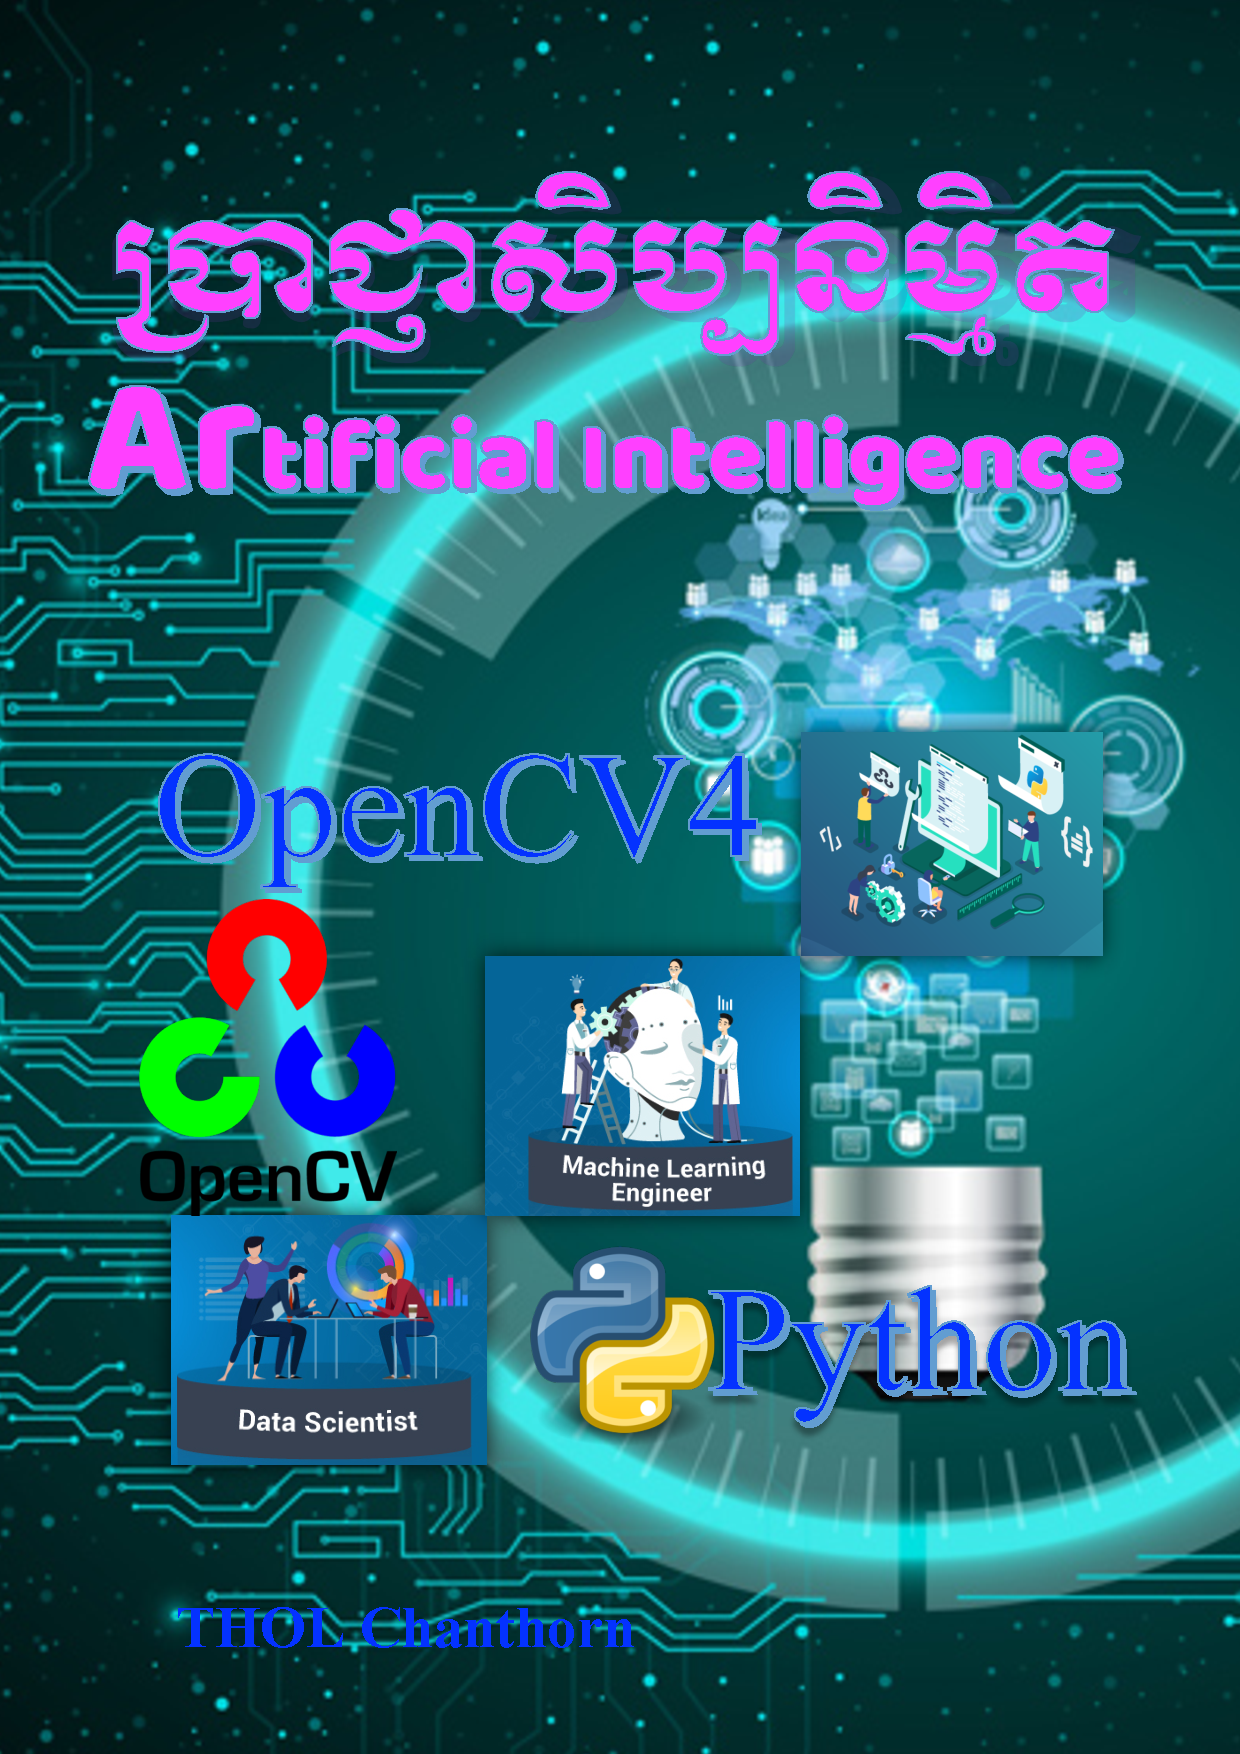
\includegraphics[width=\paperwidth]{background.pdf}};
%\draw (current page.center) node [fill=ocre!30!white,fill opacity=0.6,text opacity=1,inner sep=2cm]
%{\Huge\centering\bfseries\sffamily\parbox[c][][t]{\paperwidth}
%{\centering {\khl វិភាគអនុវត្តន៍សម្រាប់បច្ចេកវិទ្យា}{\enb OpenCV}\\[20pt] % Book title
%{\Large {\ad គណិតវិទ្យា}}\\[20pt] % Subtitle
%{\ad សម្រាប់ប្រើប្រាស់ផ្ទៃក្នុង}\\
%{\huge {\khl ថុល ចាន់ថន}}}}; % Author name
\end{tikzpicture}
\vfill
\endgroup
%----------------------------------------------------------------------------------------
%	COPYRIGHT PAGE
%----------------------------------------------------------------------------------------
\newpage
~\vfill
\thispagestyle{empty}

\noindent Copyright \copyright\ 2019 {\ad ថុល ចាន់ថន}\\ % Copyright notice
\noindent \textit{\khl រៀបរៀងលើកទី១ } % Printing/edition date
\noindent \textsc{book-website.com}\\ % URL
{\ad មុនវិជ្ជាគណិតវិភាគមានសារៈសំខាន់ក្នុងផ្នែកបច្ចេកវិទ្យាដែលវាជាទ្រឹស្តីដើម្បីបង្កើតជាអនុគមន៍}
%----------------------------------------------------------------------------------------
%	TABLE OF CONTENTS
%----------------------------------------------------------------------------------------
%\usechapterimagefalse % If you don't want to include a chapter image, use this to toggle images off - it can be enabled later with \usechapterimagetrue
\chapterimage{chapter_head_1.png} % Table of contents heading image
\pagestyle{empty} % Disable headers and footers for the following pages
\tableofcontents % Print the table of contents itself
\cleardoublepage % Forces the first chapter to start on an odd page so it's on the right side of the book
\pagestyle{fancy} % Enable headers and footers again


%	PART
%----------------------------------------------------------------------------------------
\part{\khl ផ្នែកទី១}
%----------------------------------------------------------------------------------------
%	CHAPTER 1
%----------------------------------------------------------------------------------------
\chapterimage{chapter_head_1.jpg}
\chapter{\khl មូលដ្ឋានគ្រឹះនៃកម្មវិធី {\enb Python}}%chapter 1
{\en python }{\ad ជាកម្មវិធីសរសេរភាសារបស់កុំព្យូទ័រ​ ភាសារដែលប្រើក្នុង {\en python} មិនមានភាពស្មុគស្មាញក្នុងការសរសេរឡើយ  សិស្ស}\\{\ad ដែលចង់រៀនមុខវិជ្ជាសរសេរកូដគួរតែរៀនវាដំបូង​ ។}
\section{\mb print()}\index{\mb print()}%Print() function
\begin{somebox}{\m print()}
{\ad មុខងារ\;{\m print()}\;ត្រូវបានប្រើដើម្បីបង្ហាញព័ត៌មាននៅលើអេក្រង់ហើយដើម្បីប្រើវាបានអ្នកត្រូវប្រើទម្រង់ {\m print("\;")} ។}
\end{somebox}
\begin{example}
{\ad ឥលូវយើងនឹងប្រើ {\m print} ដើម្បីបង្ហាញពាក្យថា {\en Hello,World} ។ ដើម្បីបង្ហាញបានគេគ្រាន់តែសរសេរ }\\
{\m{\mb print}({\mg "Hello,World"})}
\end{example}

\StoryNote{{\ad ការប្រើប្រាស់{\m ''}ឬ{\m "\;"}គឺដូចគ្នាសញ្ញាទាំងពីរនេះត្រូវបាន}\\
{\ad ប្រើដើម្បីបង្ហាញប្រភេទទិន្ន័យជា\;{\en string}។} }{testb}
{\ad ចូរពិនិត្យមើលការសរសេរខាងក្រោមតើវាមានន័យដូចម្តេច ?}\\
{\m {\mb print}({\mg 'I study Python'})\\
{\mb print}()\\
{\mb print}({\mg 'Python is easy'})
}\\
\newline
\newline
\newline
\tikz\node[fill=green!20!white,text width=15.8cm,align=left]{
{\m=== RESTART: /Users/macpro/Desktop/Phython lesson/lesson2.py ====}\\
{\mb I study Python
\newline
\newline
Python is easy}};\\
{\ad យើងឃើញថាបន្ទាត់ត្រូវបានរំលងមួយបន្ទាត់  ហេតុដូចនេះមុខងារ {\m print}មិនបានសរសេរអ្វីទាំងអស់គឺស្មើនឹងចុះបន្ទាត់​។}
\begin{example}
{\ad ក្នុងករណីដែលអ្នកប្រើ } $\backslash${\en n}{\ad ដើម្បីចុះបន្ទាត់នោះក៏បានដែរតែត្រូវប្រុងប្រយ័ត្ន}\\
{\m {\mb print}({\mg 'I study $\backslash $n Python'})\\
{\mb print}({\mg 'Python is easy'})
}\\
\end{example}
\tikz\node[fill=green!20!white,text width=15.8cm,align=left]{
{\m=== RESTART: /Users/macpro/Desktop/Phython lesson/lesson2.py ====}\\
{\mb I study \\
Python\\
Python is easy}};\\
{\ad ប៉ុន្តែបើអ្នកប្រើ {\en slash\; n} ពីរដងវិញវាមានន័យថាបង្ហាញ {\en $\backslash$n} មកវិញ \; បើគេចះតែធ្វើបែបនេះនោះចំនួន{\en slash\; n} និងកើនឡើង ។ }
\StoryNote{{\ad នៅក្នុងមុខងារ{\m print()}យើងក៏អាចមិនប្រើ{\m ""}}\\{\ad បានផងដែរប៉ុន្តែបានតែក្នុងករណីជាការគណនាបែប}\\{\ad គណិតវិទ្យាតែប៉ុណ្ណោះ  ។}}{testb}
\begin{example}
{\m {\mb print}(3-45+3)}
\end{example}

\shadowbox{{\en LAB}}
{\en
The print() command, which is one of the easiest directives in Python, simply prints out a line to the screen.
In your first lab:}\\{\en
•	use the print() function to print the line Hello, Python! to the screen. Use double quotes around the string;}\\{\en
•	having done that, use the print() function again, but this time print your first name;}\\{\en
•	remove the double quotes and run your code. Watch Python's reaction. What kind of error is thrown?}\\{\en
•	then, remove the parentheses, put back the double quotes, and run your code again. What kind of error is thrown this time?}\\{\en
•	experiment as much as you can. Change double quotes to single quotes, use multiple print() functions on the same line, and then on different lines. See what happens.}\\



\chapterimage{chapter_head_2.jpg} % Chapter heading image
\chapter{\khl ការដំណើង {\enb OpenCV}}
{\ad នៅក្នុងមេរៀននេះចាត់ទុកថាអ្នកបានយល់ច្បាស់ពីរបៀបដំណើងក្នុុង {\en Terminal}ដើម្បីប្រើ {\en OpenCV} អ្នកត្រូវដំឡើងវាជាមុនសិន}
\section{{\khl ប្រតិបត្តិការ}{\en (mac OS X)}}\index{{\khl ប្រតិបត្តិការ}{\en (mac OS X)}}
\begin{enumerate}
	\item{\ad បើក{\en Terminal} ដើម្បីដំឡើង {\en Homebrew}}\\
	\tikz\node[fill=green!20!white,text width=15cm,align=left]{
	/usr/bin/ruby -e "\$(curl -fsSL https://raw.githubusercontent.com/Homebrew/install/master/install)"
	};
	\item{\ad ចូលទៅកាន់វេបសាយ {\en OpenCV\;https://opencv.org} ដើម្បីដំឡើង {\en OpenCV} }
	\item{\ad ដំឡើង {\en PyCharm}{\en https://matplotlib.org/}: នៅក្នុង {\en  PyCharm} អ្នកត្រូវដំឡើង {\en numpy} និង {\en opencv-python} បន្ថែមទៀត}
	\item{\ad នៅក្នុង {\en mac OS X} មាន {\en python2} រួចហើយ  តែអ្នកត្រូវដំឡើង {\en python3} បន្ថែមទៀត}
\end{enumerate}
\section{\khl ប្រព័ន្ធកូអរដោនេក្នុង {\enb OpenCV}}\index{\ad ប្រព័ន្ធកូអរដោនេក្នុង {\enb OpenCV}}% ប្រព័ន្ធកូអរដោនេក្នុង opencv
{\ad ដើម្បីបង្ហាញប្រព័ន្ធកូអរដោនេក្នុង {\en OpenCV}និងពីរបៀប {\en access}ក្នុង {\en pixels}មួយៗ\;យើងពិនិត្យមើលទំហំរូបនៃ{\en logo}របស់}\\{\ad {\en OpenCV}ខាងក្រោម៖ }\\

\includegraphics[scale=0.4]{opencvlogo.png}\\
{\ad {\en logo} នេះមានទំហំ $20\times18$ដែលវាជារូបដែលមាន{\en pixels}ចំនួន{\en 360} ហេតុដូចនេះយើងអាចបន្ថែមប្រអប់{\en pixel}ក្នុងអ័ក្សដូចបង្ហាញខាងក្រោម៖}
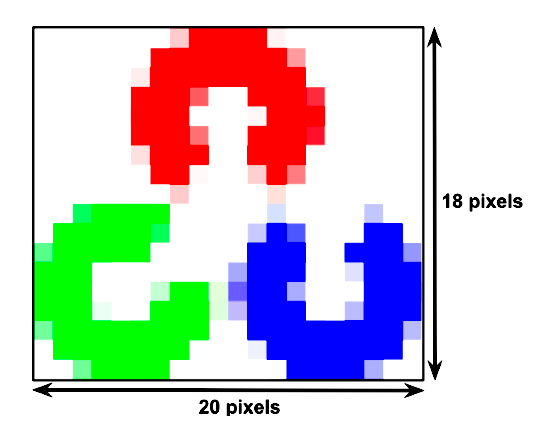
\includegraphics[scale=0.4]{opencvlogo2.png}\\
{\ad ឥលូវយើងនឹងពិនិត្យមើល{\en pixel}ក្នុងទម្រង់ $(x,y)$ដែលចាប់រាប់ពី $(0,0)$ }\\
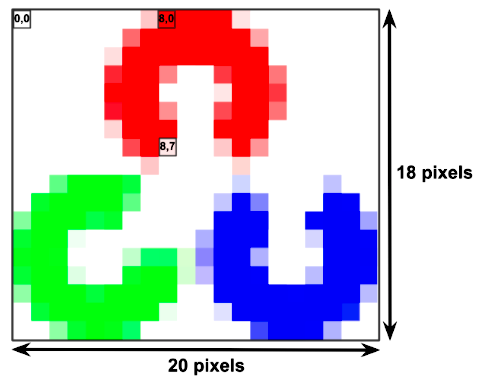
\includegraphics[scale=0.4]{opencvlogo3.png}\\
{\ad ទិន្ន័យចំពោះ {\en pixel} នីមួយៗបានមកពីរូបភាពក្នុងវិធីដូចគ្នានៃអារេដោយផ្អែកទៅលើការបង្កើតក្នុង {\en Python}}
\section{\enb Accessing and manipulating pixels in OpenCV}\index{\enb Accessing and manipulating pixels in OpenCV}%{\enb Accessing and manipulating pixels in OpenCV}

\subsection{\khl ការអានរូបភាព}\index{\ad របៀបអានរូបភាព}%ការអានយករូបភាព
{\ad រូបភាពត្រូវបានបង្ហាញជាអនុគមន៍ {\en 2D}$f(x,y)$ដែល $f(x,y)$ ជាមានកូអរដោនេជាចន្លោះ ហើយតម្លៃនៃ $f$ត្រង់ចំណុច $(x,y)$សមមាត្រទៅ}\\{\ad នឹងកម្រិតនៃការបង្ហាញពណ៌របស់រូបភាព។ម៉្យាងវិញទៀត\;ទាំងគូ $(x,y)$តម្លៃនៃពណ៌របស់ $f$ជាចំនួន{\en discrete}រាប់អស់ទាំងអស់\;រូបភាពបែប}\\{\ad នេះហៅថា"រូបភាពឌីជីថល"{\en(digital image)} ។ ដូចនេះ $f(x,y)$យកតម្លៃដូចខាងក្រោម៖}\\
\textbullet{\ad $x\in[0,h-1]:$ដែល $h$ជាកម្ពស់នៃរូបភាព}\\
\textbullet{\ad $y\in[0,w-1]:$ដែល$w$ជាប្រវែងបាតនៃរូបភាព}\\
\textbullet{\ad $f(x,y)\in[0,L-1]$ដែល $L=256${\en (for an 8-bit image)}}
\newline
{\ad ពណ៌នៃរូបភាពតាងដោយវិធីដូចគ្នា\;ប៉ុន្តែយើងត្រូវកំណត់អនុគមន៍៣ទៀតដើម្បីតាងពណ៌​ក្រហម\;ពណ៌បៃតង\;និងពណ៌ខៀវរៀងគ្នា។អនុគមន៍}\\{\ad នីយមួយៗមានរូបមន្តដូចគ្នាជា $f(x,y)$សម្រាប់កំណត់ {\en grayscale images} យើងតាង$fR(x,y),fG(x,y)$និង$fB(x,y)$}\\
{\ad រូបភាពដែលមានពណ៌ខ្មៅនិងពណ៌សគោរពតាមតម្លៃប្រហែលដូចគ្នាក្នុងវិធីនៃអនុគមន៍មួយ{\en 0(black),255(white)}}
\begin{somebox}{\en Reading Image}
{\ad យើងនឹងទាញយករូបមកអានជាទម្រង់ pixel ដែលការអាននេះគឺអានជាម៉ាទ្រីស ហើយយើងត្រូវប្រើ {\en package numpy} និង {\en cv2} ដើម្បីទាញអានយករូបបាន។}
\end{somebox}
\newpage
\StoryNote{{\ad {\red NumPy} ជា\;{\en package }សម្រាប់ការគណនាដោយប្រើ {\en Python} ។ វាមានផ្ទុកនូវមុខងារ៖}\\
$\bullet${\en Array object}{\ad ដែលមាន $N$ វិមាឌ}\\
$\bullet${\ad មានអនុគមន៍ដែលអាចផ្សាយបន្តផ្ទាល់{\en (broadcasting)}}\\
$\bullet${\en Tools}{\ad សម្រាប់បញ្ចូលគ្នាជាមួយ {\en C/C++} និងកូដ {\en Fortran}}\\
$\bullet${\ad ពីជគណិតលីនេអ៊ែរសំខាន់ៗបំប្លែង{\en Fourier}និង}\\{\ad សមត្ថភាពបង្កើតចំនួនចៃដន្យ }\\
{\red  import\;cv}\;{\ad វានឹងផ្ទុកការចងភ្ជាប់}{\en c-api}{\ad ចាស់។}\\{\en IplImage} {\ad មិនអាចប្រើបានខណៈពេលដែលវាផ្ទុកបែប}\\{\ad នេះចំពោះ}{\en api}{\ad ចាស់នឹងបញ្ជប់ភ្លាមៗជំនួសមកវិញការ}\\{\ad ប្រើប្រាស់}{\red import\;cv2}{\ad ទាញយក}{\en C++\;api}{\ad ហើយប្រើ}\\{\ad អារេ}{Numpy}{\ad សម្រាប់}{\en image}{\ad ។}}{testb}

{\m import numpy\\
{\mo import} cv2\\
img=cv2.imread('lena.jpg'{\mo,}1)\\
{\mb print}(img)\\
cv2.imshow('image'{\mo,}img)\\
cv2.waitKey(5000)\\
cv2.destroyAllwindow()}
\newline
\newline
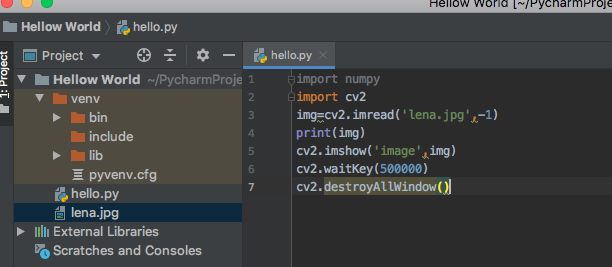
\includegraphics[scale=0.4]{readimage.png}\\
\vspace{1cm}\\
{\ad ដើម្បីទាញរូបបាន \;អ្នកត្រូវ ចូលទៅ {\en file>other settings>Preferences of New Projects...>Project Interpreter} ដើម្បីដាក់បន្ថែម {\en package} $numpy$ និង$opencv-python$  បន្ទាប់មកត្រូវ{\en copy} រូបមកដាក់ក្នុង {\en project} នេះ ដោយគ្រាន់តែ {\en past}ត្រង់{\en project}}\\

\begin{breakcode}[{\ad ដំណើរការបស់កូដ}]
\textbullet{\mb img=cv2.imread('lena.jpg',1):}{\ad អានរូបភាពដែលមានឈ្មោះ{\en lena}ដោយយកពណ៌របស់រូបភាព}\\{\ad ដើម(អាចយក {\en 1,-1,0})រូបភាពជាទម្រង់ម៉ាទ្រីសទៅដាក់ក្នុង {\en variable} {\m img}ដោយអានជា {\en pixel} ។}\\
\textbullet{\mb print(img):}{\ad បង្ហាញរូប{\en lena}លើអេក្រង់។}\\
\textbullet{\mb cv2.imshow('image',img):}{\ad បង្ហាញរូបភាពតាម}{\en variable}{\ad ដែលមានឈ្មោះថា }{\en img}\\
\textbullet{\mb cv2.waitKey(5000):}{\ad កំណត់ឱ្យរូបភាពបង្ហាញត្រឹមតែ 5វិនាទីបន្ទាប់មកវានឹងបិទការបង្ហាញ។}\\
\textbullet{\mb cv2.destroyAllwindow():}{\ad បិទផ្ទាំងកម្មវិធី}
\end{breakcode}
\subsection{\khl ការបង្ហាញវីឌីអូពីកាមរ៉ា}\index{\khl ការបង្ហាញវីឌីអូពីកាមរ៉ា}%{\khl ការបង្ហាញវីឌីអូពីកាមរ៉ា}
\begin{example}
{\ad ឥលូវខ្ញុំចង់បង្ហាញរូបភាពតាមរយៈកាមរ៉ា}\\
{\m
{\mo import} cv2\\
cap=cv2.VideoCapture({\mb 0});\\
{\mo while}({\mo True}):\\
\indent ret,frame=cap.read()\\
  \indent cv2.imshow({\mg 'frame'},frame)\\
  \indent {\mo if }cv2.waitKey({\mb 1})\&{\mb 0xFF}==ord({\mb 'q'}):\\
     \indent\indent  {\mo break}\\
cap.release()\\
cv2.destroyAllWindows()\\
}
\end{example}
\begin{breakcode}
{\mb cap=cv2.VideoCapture(0):}{\m {\ad បើកឱ្យកាមរ៉ាដំណើរការ}VideoCapture(0)\;({\ad ធម្មតា0បើវាមិន}}\\{\m {\ad ដើរគឺប្រើ-1})}{\ad មានន័យថាបើកកាមរ៉ាទី១របស់កាមរ៉ាកុំព្យូទ័រផ្ទាល់\;បើអ្នកបានតកាមរ៉ាពីកុំព្យូទ័របន្ថែមទៀតនោះអ្នកអាចដាក់}\\{\m VideoCapture(1),VideoCapture(2)}{\ad ឬច្រើនជាងនេះ\;ប៉ុន្តែអ្នកក៏អាចដាក់ភ្ជាប់ជាមួយវីឌីអូដែល}\\{\ad មានស្រាប់ដោយបន្ថែមជា}
{\en input file name}{\m VideoCapture('myvideo.avi')}\\
{\mb while(True):}{\ad ជាលក្ខ័ណដែលដាក់ឱ្យកាមរ៉ាបន្តថត}\\
{\mb ret,frame=cap.read():}{\ad នៅពេលដែល{\m cap.read()}ដំណើរការថតនោះវានឹងយកទៅដាក់ក្នុង}\\{\ad {\m frame} ហើយ {\m ret}បញ្ជាក់ថា}{\en True}{\ad ឬ}{\en False}\\
{\mb if cv2.waitKey(1)\&0xFF==ord('q'):}{\ad នៅពេលដែលអ្នកចុចអក្សរqនៅពេលដែលកំពុងថត}\\{\ad នោះវានឹងបិទកម្មវិធី}\\
{\mb break:}{\ad បិទលក្ខ័ណ}{\m while}\\
{\mb cap.release():}{\ad បង្ហាញវីឌីអូ}\\
\end{breakcode}
\StoryNote{{\mb cvtColor\;}{\ad មានន័យថា\;{\en convert color}}}{testa}
{\ad ប្រសិនបើអ្នកចង់ដាក់វីឌីអូឱ្យមានពណ៌សខ្មៅនោះនៅត្រង់{\m while}ត្រូវបន្ថែម}\\
{\m gray=cv2.cvtColor()}\\
{\ad ហើយនៅត្រង់ដូរត្រង់}{\m cv2.imshow('frame',gray)}\\
\newline
\newline
{\m while(True):\\
  \indent rat,frame=cap.read()\\
 \indent{\mo gray=cv2.cvtColor(frame,cv2.COLOR\_BGR2GRAY)}\\
    \indent {\mo cv2.imshow('frame',gray)}\\
   \indent  cv2.waitKey(1)\&0xFF==ord('q'):\\
        break}\\
  \newline
  {\ad ប្រសិនជាយើងចង់រកទំហំរបស់{\en frame} នោះយើងត្រូវប្រើ}{\m cap.get(cv2.CAP\_PROP\_FRAME\_WIDTH)}{\ad និង}\\{\m cap.get(cv2.CAP\_PROP\_FRAME\_HEIGHT)}{\ad ហើយដើម្បីបង្ហាញនៅលើផ្ទាំងកម្មវិធីអ្នកត្រូវដាក់}{\m print}{\ad អ្នក}\\{\ad អាចប្រើមុខងារផ្សេងៗបន្ថែមទៀតដោយចូលទៅ}\;\url{https://shorturl.at/dNPZ2}{\ad ដើម្បីអានបន្ថែម}\\
  \newline
{\m while(True):\\
  \indent rat,frame=cap.read()\\
  \indent {\mo print(cap.get(cv2.CAP\_PROP\_FRAME\_WIDTH))}\\
  \indent {\mo print(cap.get(cv2.CAP\_PROP\_FRAME\_HEIGHT))}\\
 \indent gray=cv2.cvtColor(frame,cv2.COLOR\_BGR2GRAY)\\
    \indent  cv2.imshow('frame',gray)\\
   \indent  cv2.waitKey(1)\&0xFF==ord('q'):\\
        break}\\
 \subsection{\enb Saving Video Live Stream}\index{\enb Saving Video Live Stream}%{\enb Saving Video Live Stream}
 
 \begin{example}
 {\ad ដើម្បីរកទុកវីឌីអូដែលយើងបានថតនោះយើងត្រូវ}\\
 \textbullet{\ad បង្កើត{\en \;VideoWriterClass}\;នៅក្នុង{\en \; Class}នេះត្រូវមាន\;{\en argument}៣ដែលទី១ជាឈ្មោះនិងប្រភេទ{\en file}\;{\en argument}ទី២គឺ}\\{\ad មានមុខងារដែលអាចបំប្លែងវីឌីអូនេះបានដោយយើងនឹងប្រើ\;{\en forecc}ហើយ\;{\en argument}ទី៣គឺល្បឿនរបស់\;{\en frame}}\\
 \textbullet{\ad នៅក្នុង{\en \;while loop} មានអញ្ញាត{\m\; frame}និង {\m ret}នៅពេលដែល{\m frame}ពិតនោះ\;{\m ret} មិនពិតហើយ\;{\m ret} ជាអញ្ញាត {\en boolean}។ យើងដាក់លក្ខ័ណថាបើ{\m\; ret} ពិតនោះឱ្យ{\m \;write}វីឌីអូទៅតាម{\m \;frame}}\\
 \textbullet{\ad ចុងក្រោយគឺបន្ថែម{\m \;out.release()}}\\
 \newline
 {\m
 {\mo import} cv2\\
cap = cv2.VideoCapture({\mb 0})\\
fourcc = cv2.VideoWriter\_fourcc(*{\mg 'XVID'})\\
save = cv2.VideoWriter({\mg 'output.avi'}{\mo ,} fourcc{\mo ,}{\mb 20.0}{\mo ,} ({\mb 640}{\mo ,}{\mb 480}))\\
{\mb print}(cap.isOpened())\\
{\mo while}(cap.isOpened()):\\
\indent ret{\mo ,}frame = cap.read()\\
\indent{\mo if }ret =={\mo True}:\\
      \indent\indent{\mb print}(cap.get(cv2.CAP\_PROP\_FRAME\_WIDTH))\\
       \indent\indent{\mb print}(cap.get(cv2.CAP\_PROP\_FRAME\_HEIGHT))\\
      \indent\indent save.write(frame)\\
       \indent\indent gray = cv2.cvtColor(frame{\mo ,} cv2.COLOR\_BGR2GRAY)\\
       \indent\indent cv2.imshow({\mg 'frame'}{\mo , }gray)\\
     \indent\indent{\mo  if }cv2.waitKey({\mb 1}) \& {\mb 0xFF} == {\mb ord}({\mg 'q'}):\\
        \indent\indent\indent {\mo break}\\
   \indent\indent {\mo else}:\\
     \indent\indent\indent {\mo break}\\
cap.release()\\
save.release()\\
cv2.destroyAllWindows()}
 \end{example}
 {\ad នៅពេលដែលយើង {\en run}កូដហើយនោះវាចាប់ផ្តើមថតយកវីឌីអូ\;នៅពេលយើងបិទកម្មវិធី(ចុះអក្សរ\;q ឬចុច\;stop)យើងឃើញថា}\\{\ad កូដនេះគឺយកតាមកូដក្នុងឧទាហរណ៍មុន ។}
 \section{\enb Drawing Shap}\index{\enb Drawing Shap}%{\enb Drawing Shap}
 {\ad នៅក្នុងចំណុចនេះយើងនឹងរៀនពីការគូររូបធរណីមាត្រមួយចំនួន}
 {\m 
{\mo import }numpy {\mo as} np\\
{\mo import }cv2\\

\#img = cv2.imread('lena.jpg', 1)\\
img = np.zeros([512{\mo,} 512{\mo,} 3]{\mo , }np.uint8)\\

img = cv2.line(img{\mo, }(0,0){\mo, }(255,255){\mo , }(147{\mo, }96{\mo, }44){\mo, }10) \# 44, 96, 147\\
img = cv2.arrowedLine(img{\mo, }(0{\mo ,}255){\mo , }(255{\mo,}255){\mo, }(255{\mo, }0{\mo, }0){\mo, }10)\\
img = cv2.rectangle(img{\mo, }(384{\mo, }0){\mo, }(510{\mo, }128){\mo , }(0{\mo , }0{\mo, }255){\mo , }10)\\
img = cv2.circle(img{\mo, }(447{\mo, }63){\mo, }63{\mo, }(0{\mo, }255{\mo, }0){\mo,} -1)\\
font = cv2.FONT\_HERSHEY\_SIMPLEX\\
img = cv2.putText(img{\mo,}{\mg'OpenCv'}{\mo, }(10{\mo, }500){\mo, }font{\mo, }4{\mo,} (0{\mo,} 255{\mo,} 255){\mo, }10{\mo, }cv2.LINE\_AA)\\
img = cv2.ellipse(img{\mo,}(256{\mo,}256){\mo,}(100{\mo,}50){\mo,}0{\mo,}0{\mo,}180{\mo,}255{\mo,}-1)\\

pts = np.array([[10{\mo,}5]{\mo,}[20{\mo,}30]{\mo,}[70{\mo,}20]{\mo,}[50{\mo,}10]]{\mo,} np.int32)\\
pts = pts.reshape((-1{\mo,}1{\mo,}2))\\
img = cv2.polylines(img{\mo,}[pts]{\mo,}{\mo True}{\mo,}(0{\mo,}255{\mo,}255))\\
cv2.imshow({\mg'image'}{\mo, }img)\\
cv2.waitKey({\mb 0})\\
cv2.destroyAllWindows()}
 
 
\chapterimage{chapter_head_3.jpg}
\chapter{{\khl លំហបាណាក}}


%----------------------------------------------------------------------------------------
%	PART
%----------------------------------------------------------------------------------------
\part{\khl ផ្នែកទី២}
%----------------------------------------------------------------------------------------
%	CHAPTER 3
%----------------------------------------------------------------------------------------
\chapterimage{chapter_head_1b.png} % Chapter heading image
\chapter{\enb​ Processing and  OpenCV}
\chapterimage{chapter_head_2b.jpg} % Chapter heading image
\chapter{\khl​ ប្រភពរូបភាពនិងការតាង}

\begin{itemize}
\item{\ad មូលដ្ឋាគ្រឹះនៃរូបភាពឌីជីថល}
\item{\ad រូបភាពក្នុង Processing}
\item{\ad រូបភាពផ្លាស់ទីក្នុង Processing}
\item{\ad រូបភាពម៉ាទ្រីសក្នុង OpenCV}
\item{\ad ការបម្លែងរូបភាពរវាង ​Processing និង OpenCV}
\end{itemize}
\section{{\khl មូលដ្ឋាគ្រឹះនៃរូបភាពឌីជីថល}{\enb Digital Image Fundamentals}}\index{{\khl មូលដ្ឋាគ្រឹះនៃរូបភាពឌីជីថល}{\enb Digital Image Fundamentals}}%មូលដ្ឋាគ្រឹះនៃរូបភាពឌីជីថល


%----------------------------------------------------------------------------------------
%	BIBLIOGRAPHY
%----------------------------------------------------------------------------------------
\chapter*{Bibliography}
\addcontentsline{toc}{chapter}{\textcolor{ocre}{Bibliography}} % Add a Bibliography heading to the table of contents
%------------------------------------------------
\section*{Articles}
\addcontentsline{toc}{section}{Articles}
\printbibliography[heading=bibempty,type=article]
%------------------------------------------------
\section*{Books}
\addcontentsline{toc}{section}{Books}
\printbibliography[heading=bibempty,type=book]
%----------------------------------------------------------------------------------------
%	INDEX
%----------------------------------------------------------------------------------------
\cleardoublepage % Make sure the index starts on an odd (right side) page
\phantomsection
\setlength{\columnsep}{0.75cm} % Space between the 2 columns of the index
\addcontentsline{toc}{chapter}{\textcolor{ocre}{Index}} % Add an Index heading to the table of contents
\printindex % Output the index
%----------------------------------------------------------------------------------------
\end{document}
